\documentclass{beamer}
%
% Choose how your presentation looks.
%
% For more themes, color themes and font themes, see:
% http://deic.uab.es/~iblanes/beamer_gallery/index_by_theme.html
%
\mode<presentation>
{
  \usetheme{default}      % or try Darmstadt, Madrid, Warsaw, ...
  \usecolortheme{crane} % or try albatross, beaver, crane, ...
  \usefonttheme{structurebold}  % or try serif, structurebold, ...
  \setbeamertemplate{navigation symbols}{}
  \setbeamertemplate{caption}[numbered]
} 

\usepackage[english]{babel}
\usepackage[utf8x]{inputenc}

\title[ML]{Machine Learning}
\author{Pawel Wocjan}
\institute{University of Central Florida}
\date{Spring 2019}

\begin{document}

\begin{frame}
  \titlepage
\end{frame}

\begin{frame}{Sources for Slides}

\begin{itemize}
\item I have extensively used the machine learning materials that have been prepared by Google. 

\medskip
\footnotesize{ 
\url{https://developers.google.com/machine-learning/crash-course/}
}

\item Google has licensed these materials under the Creative Commons Attribution 3.0 License.

\medskip
\footnotesize{ 
\url{https://creativecommons.org/licenses/by/3.0/}
}
\end{itemize}
\end{frame}

% Uncomment these lines for an automatically generated outline.
\begin{frame}{Outline}
  \tableofcontents
\end{frame}

\section{Generalization}

\subsection{Peril of Overfitting}

\begin{frame}{Peril of Overfitting}
\begin{itemize}
    \item To gain some intuition about generalization, let's look at the following three figures. 
    \item Assume that each dot in these figures represents a tree's position in a forest. The two colors have the following meanings:
    \begin{itemize}
        \item The blue dots represent sick trees.
        \item The orange dots represent healthy trees.
    \end{itemize}
    \item Can you imagine a good model for predicting subsequent sick or healthy trees? 
    \item Take a moment to mentally draw an arc that divides the blues from the oranges, or mentally lasso a batch of oranges or blues. 
\end{itemize}
\end{frame}

\begin{frame}{Peril of Overfitting}
\includegraphics[width=0.75\textwidth]{images/GeneralizationA.png}
\end{frame}

\begin{frame}{Peril of Overfitting}
\begin{itemize}
\item Look now at the next figure, which shows how a certain machine learning model separated the sick trees from the healthy trees. 
\item Note that this model produced a very low loss.
\end{itemize}
\end{frame}

\begin{frame}{Peril of Overfitting}
\includegraphics[width=0.75\textwidth]{images/GeneralizationB.png}
\end{frame}

\begin{frame}{Peril of Overfitting}
\begin{itemize}
\item At first glance, this model appears to do an excellent job of separating the healthy trees from the sick ones. Or does it?
\end{itemize}
\end{frame}

\begin{frame}{Peril of Overfitting}
\begin{itemize}
\item The next figure shows what happened when we added new data to the model. 
\item It turned out that the model adapted very poorly to the new data. 
\item Notice that the model miscategorized much of the new data.
\end{itemize}
\end{frame}

\begin{frame}{Peril of Overfitting}
\includegraphics[width=0.75\textwidth]{images/GeneralizationC.png}
\end{frame}

\begin{frame}{Peril of Overfitting}
\begin{itemize}
\item The model shown did a bad job predicting new data.
\item This {\bf overfits} the peculiarities of the data it trained on. 
\item An overfit model gets a low loss during training but does a poor job predicting new data. 
\item If a model fits the current sample well, how can we trust that it will make good predictions on new data? 
\item As you'll see later on, overfitting is caused by making a model more complex than necessary. 
\item The fundamental tension of machine learning is between fitting our data well, but also fitting the data as simply as possible.
\end{itemize}
\end{frame}

\begin{frame}{Peril of Overfitting}
\begin{itemize}
\item Machine learning's goal is to predict well on new data drawn from a (hidden) true probability distribution. 
\item Unfortunately, the model can't see the whole truth; the model can only sample from a training data set. 
\item If a model fits the current examples well, how can you trust the model will also make good predictions on never-before-seen examples?
\end{itemize}
\end{frame}

\begin{frame}{Peril of Overfitting}
\begin{itemize}
    \item William of Ockham, a 14th century friar and philosopher, loved simplicity. 
    \item He believed that scientists should prefer simpler formulas or theories over more complex ones. 
    \item To put {\bf Ockham's razor} in machine learning terms:
    
    \medskip
    \emph{The less complex an ML model, the more likely that a good empirical result is not just due to the peculiarities of the sample.}
\end{itemize}
\end{frame}

\begin{frame}{Peril of Overfitting}
\begin{itemize}
    \item In modern times, we've formalized Ockham's razor into the fields of statistical learning theory and computational learning theory. 
    \item These fields have developed generalization bounds -- a statistical description of a model's ability to generalize to new data based on factors such as:
    \begin{itemize}
        \item the complexity of the model
        \item the model's performance on training data
    \end{itemize}
    For instance, take a look at VC-dimension:
    {\footnotesize \url{https://en.wikipedia.org/wiki/Vapnik-Chervonenkis\_dimension}}
    \item While the theoretical analysis provides formal guarantees under idealized assumptions, they can be difficult to apply in practice. 
    \item In our course, we focus instead on empirical evaluation to judge a model's ability to generalize to new data.
\end{itemize}
\end{frame}

\begin{frame}{Peril of Overfitting}
\begin{itemize}
    \item A machine learning model aims to make good predictions on new, previously unseen data. 
    \item But if you are building a model from your data set, how would you get the previously unseen data? 
    \item Well, one way is to divide your data set into two subsets:
    \begin{itemize}
        \item {\bf training set} -- a subset to train a model
        \item {\bf test set} -- a subset to test the model
    \end{itemize}
    \item Good performance on the test set is a useful indicator of good performance on the new data in general, assuming that:
    \begin{itemize}
        \item The test set is large enough.
        \item You don't cheat by using the same test set over and over.
    \end{itemize}
\end{itemize}
\end{frame}

\begin{frame}{Peril of Overfitting}
\begin{itemize}
    \item The following three basic assumptions guide generalization:
    \begin{itemize}
        \item We draw examples {\bf independently and identically (i.i.d)} at random from the distribution. In other words, examples don't influence each other. 
        
        An alternate explanation: i.i.d. is a way of referring to the randomness of variables.
        \item The distribution is {\bf stationary}; that is the distribution doesn't change within the data set.
        \item We draw examples from partitions from the {\bf same distribution}.
    \end{itemize}
\end{itemize}
\end{frame}

\begin{frame}{Perils of Overfitting}
\begin{itemize}
    \item In practice, we sometimes violate these assumptions. For example:
    \begin{itemize}
        \item Consider a model that chooses ads to display. The i.i.d. assumption would be violated if the model bases its choice of ads, in part, on what ads the user has previously seen.
        \item Consider a data set that contains retail sales information for a year. User's purchases change seasonally, which would violate stationarity.
        \item When we know that any of the preceding three basic assumptions are violated, we must pay careful attention to metrics.
    \end{itemize}
    \item When we know that any of the preceding three basic assumptions are violated, we must pay careful attention to metrics.
\end{itemize}
\end{frame}

\begin{frame}{Summary}
\begin{itemize}
    \item Overfitting occurs when a model tries to fit the training data so closely that it does not generalize well to new data.
    \item If the key assumptions of supervised ML are not met, then we lose important theoretical guarantees on our ability to predict on new data.
\end{itemize}
\end{frame}

\begin{frame}{Key Terms}
\begin{itemize}
    \item generalization
    \item overfitting
\item prediction
\item stationarity
\item test set
\item training set

\end{itemize}
\end{frame}

\section{Training and Test Sets}

\subsection{Splitting Data}

\begin{frame}{Splitting Data}
\begin{itemize}
    \item We have introduced the idea of dividing the data set into two subsets:
    \begin{itemize}
        \item training set—a subset to train a model.
        \item test set—a subset to test the trained model.
    \end{itemize}
    \item You could imagine slicing the single data set as follows:
    
    \medskip
    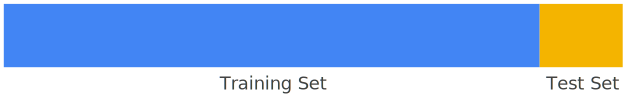
\includegraphics[width=0.9\textwidth]{images/PartitionTwoSets.png}
\end{itemize}
\end{frame}

\begin{frame}{Splitting Data}
\begin{itemize}
    \item Make sure that your test set meets the following two conditions:
    \begin{itemize}
        \item Is large enough to yield statistically meaningful results.
        \item Is representative of the data set as a whole. In other words, don't pick a test set with different characteristics than the training set.
    \end{itemize}
    \item Assuming that your test set meets the preceding two conditions, your goal is to create a model that generalizes well to new data. Our test set serves as a proxy for new data. 
\end{itemize}
\end{frame}

\begin{frame}{Splitting Data}
\begin{itemize}
    \item For example, consider the following figure. 
\end{itemize}
\medskip
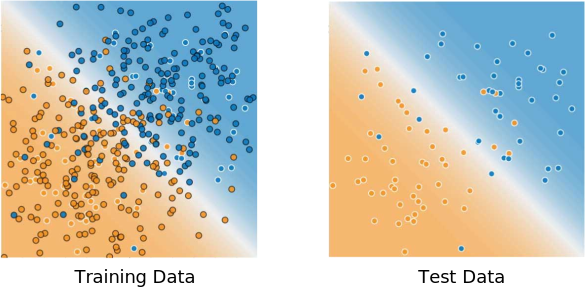
\includegraphics[width=1.0\textwidth]{images/TrainingDataVsTestData.png}
\end{frame}

\begin{frame}{Splitting Data}
\begin{itemize}
    \item Notice that the model learned for the training data is very simple. 
    \item This model doesn't do a perfect job -- a few predictions are wrong. 
    \item However, this model does about as well on the test data as it does on the training data. \item In other words, this simple model does not overfit the training data.
\end{itemize}
\end{frame}

\begin{frame}{Splitting Data}
\begin{itemize}
    \item {\bf Never} train on test data. If you are seeing surprisingly good results on your evaluation metrics, it might be a sign that you are accidentally training on the test set. 
    \item For example, high accuracy might indicate that test data has leaked into the training set.
\end{itemize}
\end{frame}

\begin{frame}{Splitting Data}
\begin{itemize}
    \item For example, consider a model that predicts whether an email is spam, using the subject line, email body, and sender's email address as features. 
    \item We apportion the data into training and test sets, with an $80$-$20$ split. After training, the model achieves $99\%$ precision on both the training set and the test set. 
    \item We'd expect a lower precision on the test set, so we take another look at the data and discover that many of the examples in the test set are duplicates of examples in the training set (we neglected to scrub duplicate entries for the same spam email from our input database before splitting the data). 
    \item We've inadvertently trained on some of our test data, and as a result, we're no longer accurately measuring how well our model generalizes to new data.
\end{itemize}
\end{frame}

\begin{frame}{Key Terms}
\begin{itemize}
    \item overfitting
    \item test set
    \item training sets
\end{itemize}
\end{frame}

\end{document}